\section{Experimental Setup}


\subsection{Physical simulators}
For our experiments, we generate tasks following the \name{} pipeline for three simple simulators:
\begin{itemize}[leftmargin=*,topsep=3pt,nosep]
    \item \texttt{BallDrop}: a ball moving vertically under gravity and bouncing on a ground surface.
    \item \texttt{DampedMassBetweenWalls}: a damped mass moving along a tilted one-dimensional track and colliding with two rigid walls.
    \item \texttt{InclinedPlane}: a mass moving along a tilted plane with a force applied periodically.
\end{itemize}
Each simulator is implemented in Simulink.
For each environment \(e\), we define two environment-specific noise scales  \(\kappa_{\mathrm{low}}^{(e)}\) and \(\kappa_{\mathrm{high}}^{(e)} = 4\kappa_{\mathrm{low}}^{(e)}\) to create two different noise regimes. 
We also consider two textual-context levels: \(D_{\text{high}}\) and \(D_{\text{none}}\), where the textual description describes the physical system, observed channels, and candidate root-cause parameters for \(D_{\text{high}}\), while the agent receives only the task description and anonymized labels for \(D_{\text{none}}\).
We report the resulting per-channel SNRs, representative noisy time-series observations, and the textual descriptions for each textual-context level in Appendix~\ref{app:environment-catalog}.

\subsection{Metrics}
We score agentic submissions based on top-1 accuracy.
For top-1 accuracy, we compare the first label predicted by the agent against the ground truth label.

For $\mathcal{I}_{\mathrm{direct}}$ tasks, performance is evaluated on the episode batch, i.e., the test files visible to the agent. 
For $\mathcal{I}_{\mathrm{code}}$ tasks, we report performance on both the episode batch and a held-out batch of additional samples. 

Random chance is the macro-average of uniform guessing over the three simulator label spaces, approximately 0.18.
Table entries report mean accuracy across seeds and simulators, with standard deviation computed over seeds.
\subsection{Agent models}
We evaluate a set of closed- and open-weight agents using their corresponding terminal-based execution platforms.
Specifically, we evaluated \texttt{gpt-5.5}, \texttt{gemini-3.1-pro-preview}, \texttt{claude-opus-4-6} and \texttt{minimax-m2.7}.
For models that expose a reasoning-effort setting, we use the high setting for all experiments.
All agents are evaluated under the same task interface, file layout, and scoring procedure.
The full list of agent profiles, platform commands, available tools, and token-cost metadata is provided in the appendix.

\subsection{Runtime environment}
Each evaluation episode is executed in an isolated containerized environment with a timeout of one hour.
The agent has access to the task prompt, the sample files, and a Python environment with standard scientific libraries such as NumPy, pandas, SciPy, scikit-learn, and matplotlib.
The full list is provided in the appendix. 
The agent may run terminal commands and Python scripts to inspect, transform, or visualize the time series. 
Internet access is disabled.

An episode ends when the agent returns control to the harness or when the one-hour timeout is reached.
For direct-prediction tasks, the required final artifact is \texttt{results.json}.
For code-rule tasks, the required final artifact is \texttt{rule.py}.
If the required artifact is missing or invalid, or if the submitted \texttt{rule.py} cannot be executed by the harness, the episode receives a score of zero for the entire batch.
Episodes terminated by the one-hour timeout are excluded from aggregate accuracy and reported separately, together with infrastructure-related failures such as API outages, platform interruptions, and container initialization failures.

\subsection{Experimental design}
Each experiment is defined by its test set and its controllable factors, namely the noise regime, the task interface, the number of labeled examples, and the textual-context level.
To support controlled comparisons across textual-context and observation conditions, matched experimental conditions use the same test samples.
This pairing ensures that differences between conditions reflect changes in one of the controllable factors rather than changes in the underlying test samples.
Each test batch contains \(B=10\) samples. When \(B\) is not divisible by the number of label classes in an environment, test batches are balanced as evenly as possible, so that any two class counts differ by at most one sample.

Our main experiment evaluates a grid over \(\{\kappa_{\mathrm{low}}, \kappa_{\mathrm{high}}\} \times \{\mathcal{I}_{\mathrm{direct}}, \mathcal{I}_{\mathrm{code}}\}\), using three labeled samples per class and a high-detail textual description.
Each experiment is repeated five different times for each physical simulator.
This yields 60 evaluation episodes per agent: 15 episodes for each of the four conditions, corresponding to 150 visible test samples per condition.
We then perform two additional ablations over textual context and the number of labeled time-series examples while keeping \(\kappa_{\mathrm{high}}\) fixed for both \(\mathcal{I}_{\mathrm{direct}}\) and \(\mathcal{I}_{\mathrm{code}}\).
Due to cost constraints, we evaluate these two ablations only with \texttt{gpt-5.5} and \texttt{gemini-3.1-pro-preview}.

We present the aggregate analysis in the following sections and provide per-environment results in Appendix~\ref{app:calibration-result-tables}.

The examples of the prompts in the different settings are provided in \Cref{app:prompt-example-combinations}.


\section{Results}
\subsection{Main results}
Table~\ref{tab:acc_main_experiment_table} shows the accuracy averaged over seeds and simulators for each condition. 
Note that \texttt{claude-opus-4-6} could not be evaluated on \((\kappa_{\mathrm{high}}, \mathcal{I}_{\mathrm{code}})\) with \texttt{DampedMassBetweenWalls} because its run lasted longer than one hour.
\texttt{gpt-5.5} and \texttt{claude-opus-4-6} are the strongest performers, followed by \texttt{gemini-3.1-pro-preview}. 
By contrast, \texttt{minimax-m2.7} performs substantially worse.  While \texttt{minimax-m2.7} is strong on agentic software-engineering benchmarks such as SWE-Pro and Terminal Bench 2~\citep{minimax_m27_report_2026}, its poor performance on \name{} suggests that data-analysis requires a skills set that does is not covered by these benchmarks.

Performance decreases as noise increases from \(\kappa_{\mathrm{low}}\) to \(\kappa_{\mathrm{high}}\).
\texttt{gemini-3.1-pro-preview} is the most sensitive to noise with a drop of 16.7 percentage points.

The \(\mathcal{I}_{\mathrm{code}}\) episode accuracy is worse than direct prediction \(\mathcal{I}_{\mathrm{direct}}\), indicating a gap between recognizing diagnostic patterns in a batch of time-series observations and encoding them as a reusable rule.
Additionally, the held-out accuracy is often lower than episode accuracy, suggesting that rules fitted during exploration may not always capture stable physical signatures of the intervention

\begin{table}[ht]
\centering
\caption{Top-1 accuracy for the main experiment, aggregated across simulators.
\texttt{Episode} refers to accuracy measured on the visible test samples in the episode batch.
\texttt{Held-out} refers to accuracy measured on additional samples that are not visible to the agent during the episode.
}
\label{tab:acc_main_experiment_table}
\begingroup
\small
\newcommand{\scorepm}[2]{$#1\,{\scriptstyle\pm #2}$}

\setlength{\tabcolsep}{1.5pt}
\setlength{\aboverulesep}{0pt}
\setlength{\belowrulesep}{2pt}
\renewcommand{\arraystretch}{1.05}

\begin{tabular*}{\textwidth}{@{\extracolsep{\fill}}lcccccc@{}}
\toprule
& \multicolumn{3}{c}{\textbf{\texttt{Noise:} \texttt{low}}}
& \multicolumn{3}{c}{\textbf{\texttt{Noise:} \texttt{high}}} \\
\cmidrule(lr){2-4}\cmidrule(lr){5-7}
& \multicolumn{1}{c}{\texttt{Direct}}
& \multicolumn{2}{c}{\texttt{Code}}
& \multicolumn{1}{c}{\texttt{Direct}}
& \multicolumn{2}{c}{\texttt{Code}} \\
\cmidrule(lr){2-2}\cmidrule(lr){3-4}
\cmidrule(lr){5-5}\cmidrule(lr){6-7}
& \texttt{Episode}
& \texttt{Episode}
& \texttt{Held-out}
& \texttt{Episode}
& \texttt{Episode}
& \texttt{Held-out} \\
\midrule
\texttt{gpt-5.5}
& \scorepm{0.933}{0.09}
& \scorepm{0.853}{0.146}
& \scorepm{0.798}{0.106}
& \scorepm{0.833}{0.199}
& \scorepm{0.733}{0.238}
& \scorepm{0.665}{0.168} \\

\texttt{gemini-3.1-pro-preview}
& \scorepm{0.76}{0.164}
& \scorepm{0.733}{0.154}
& \scorepm{0.684}{0.139}
& \scorepm{0.56}{0.259}
& \scorepm{0.547}{0.196}
& \scorepm{0.57}{0.184} \\

\texttt{claude-opus-4-6}
& \scorepm{0.853}{0.125}
& \scorepm{0.687}{0.136}
& \scorepm{0.702}{0.133}
& \scorepm{0.64}{0.272}
& \scorepm{0.0}{0.0}
& \scorepm{0.0}{0.0} \\

\texttt{minimax-m2.7}
& \scorepm{0.293}{0.225}
& \scorepm{0.28}{0.193}
& \scorepm{0.353}{0.212}
& \scorepm{0.307}{0.227}
& \scorepm{0.364}{0.217}
& \scorepm{0.351}{0.218} \\
\bottomrule
\end{tabular*}
\endgroup

\end{table}

\FloatBarrier

\paragraph{More tool use does not reliably improve accuracy}
We analysed the agentic rollout to explore correlation between the accuracy and exploration and reasoning.
Fig. \ref{fig:accuracy-vs-compute} shows the accuracy on the y-axis plotted against cumulative token usage and python calls.
As shown, more exploration or longer agent rollouts do not lead to better outcomes. 
On the contrary there is a negative correlation.
Weaker agents often spend more steps running generic analyses, while stronger agents spend fewer steps constructing targeted diagnostics.



\begin{figure}[ht]
\centering
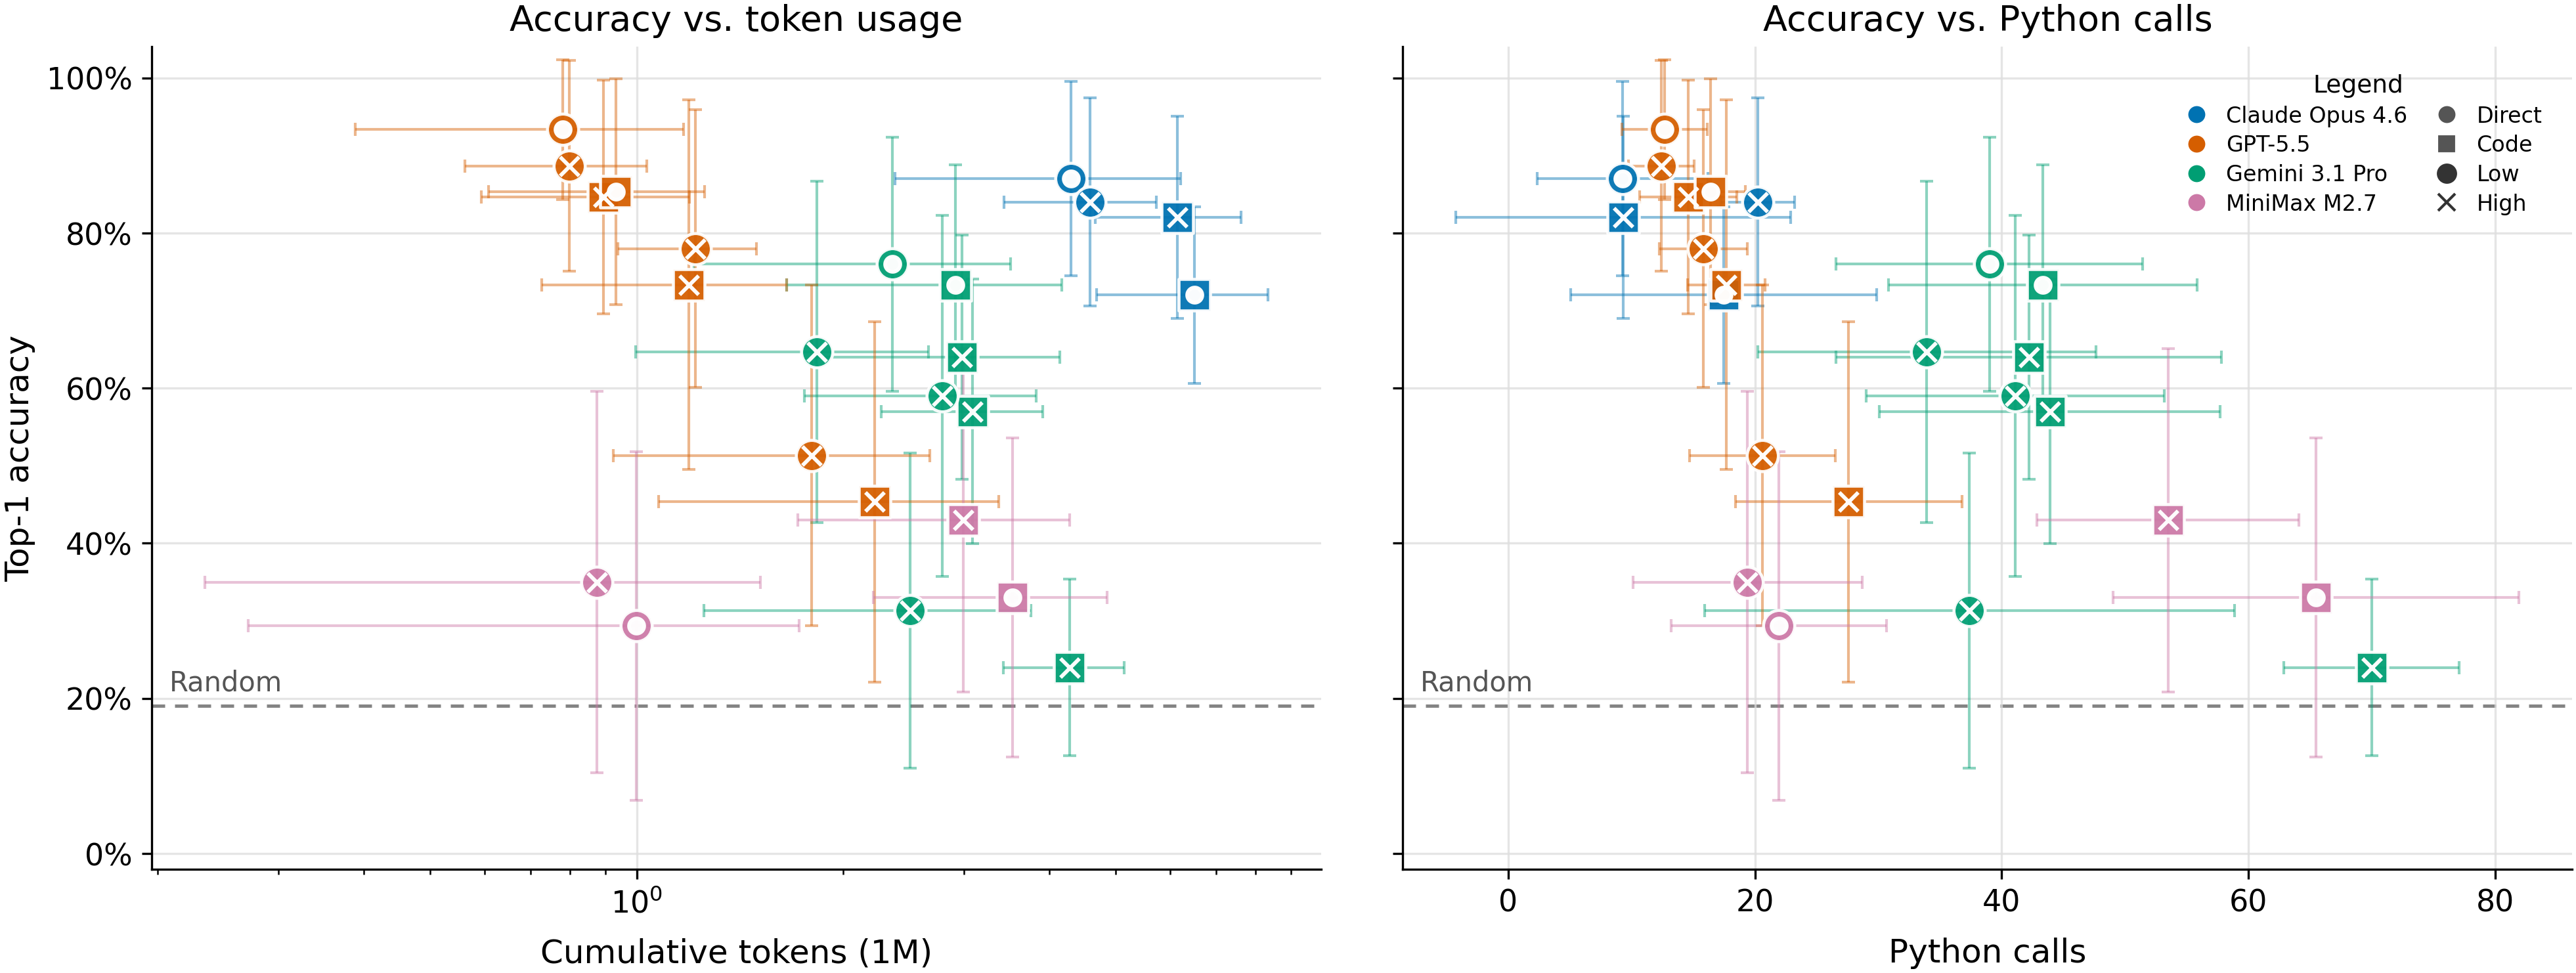
\includegraphics[width=\linewidth]{pictures/accuracy_vs_tokens_and_python_calls.pdf}
\caption{Top-1 accuracy as a function of cumulative token usage (left) and Python calls (right) for the results in the main table. 
    Each point aggregates one agent and experimental condition across completed seeds and environments; horizontal and vertical bars show standard deviation across runs.}
\label{fig:accuracy-vs-compute}
\end{figure}


Table~\ref{tab:cum-main-experiment-table} reports cumulative token usage in millions of tokens for the main experiment.

Token usage varies substantially by model and interface: \texttt{gpt-5.5} uses the fewest tokens, ranging from 0.78M--0.98M in direct mode and 0.93M--1.19M in code mode, while \texttt{claude-opus-4-6} uses the most, reaching 4.39M--4.51M tokens in direct mode and 6.59M--6.63M in code mode.
Overall while both \texttt{GPT-5.5} and \texttt{claude-opus-4-6} are on the same level of performance on the task, \texttt{claude-opus-4-6} uses many more tokens to solve them.
Across agents, code-rule tasks require more tokens than direct classification in both noise regimes.
This increase is especially visible for \texttt{claude-opus-4-6} and \texttt{minimax-m2.7}, where code-mode runs require roughly 1.5--3.6M more tokens than direct runs, indicating that writing and validating executable decision rules adds substantial interaction cost.
Higher observation noise also partially increases token usage for \texttt{GPT-5.5} and \texttt{gemini-3.1-pro-preview}, but not uniformly for \texttt{claude-opus-4-6} and  \texttt{minimax-m2.7}.




\begin{table}[ht]
\centering
\caption{Cumulative token usage for the main experiment, in millions of tokens.}
\label{tab:cum-main-experiment-table}
\begingroup
\small
\newcommand{\scorepm}[2]{$#1\,{\scriptstyle\pm #2}$}

\setlength{\tabcolsep}{5pt}
\setlength{\aboverulesep}{0pt}
\setlength{\belowrulesep}{2pt}
\renewcommand{\arraystretch}{1.05}

\begin{tabular*}{\textwidth}{@{\extracolsep{\fill}}lcccc@{}}
\toprule
& \multicolumn{2}{c}{\textbf{\texttt{Noise:} \texttt{low}}}
& \multicolumn{2}{c}{\textbf{\texttt{Noise:} \texttt{high}}} \\
\cmidrule(lr){2-3}\cmidrule(lr){4-5}
& \texttt{Direct}
& \texttt{Code}
& \texttt{Direct}
& \texttt{Code} \\
\midrule
\texttt{gpt-5.5} & \scorepm{0.78}{0.391} & \scorepm{0.932}{0.325} & \scorepm{0.975}{0.35} & \scorepm{1.191}{0.465} \\
\texttt{gemini-3.1-pro-preview} & \scorepm{2.362}{1.151} & \scorepm{2.915}{1.261} & \scorepm{2.796}{1.102} & \scorepm{3.687}{1.767} \\
\texttt{claude-opus-4-6} & \scorepm{4.386}{1.75} & \scorepm{6.585}{2.191} & \scorepm{4.505}{1.039} & \scorepm{6.628}{1.302} \\
\texttt{minimax-m2.7} & \scorepm{0.999}{0.728} & \scorepm{3.589}{1.208} & \scorepm{0.841}{0.57} & \scorepm{3.04}{1.148} \\
\bottomrule
\end{tabular*}
\endgroup

\end{table}
\FloatBarrier

\paragraph{Do agents visualise time-series observations?}
Plotting is often a primary method for data inspection. 
We quantitatively measure for each agent the number of plots generated and consumed for all the agents that support image modality. 
Surprisingly, only \texttt{GPT-5.5} uses plotting to gain insights, although sparingly in only seven different evaluation over the total of our experiments.
\texttt{gemini-3.1-pro-preview} generates plots much more frequently, with 183 plot artifacts, but never invoked an image-viewing tool in the uploaded runs. 
\texttt{claude-opus-4-6} generates no plot artifacts in the uploaded agent rollouts. 
Thus, current agents mostly explore TSENV through script-mediated summaries, feature extraction, correlations, changepoint checks, and train-set diagnostics, rather than through sustained visual inspection of the time series.





\subsection{Ablations: Labeled examples and textual context have opposite effects}
Table~\ref{tab:acc_ablation_training_examples} shows the results for the two ablations.
The left block removes the labeled examples while keeping the high-detail textual description, whereas the right block removes the high-detail textual description while keeping three labeled examples per class.
The prompts are provided in Appendix~\ref{app:prompt-example-combinations}.
Removing textual context has a large impact, decreasing performance by 28.9 and 22.6 percentage points for \texttt{gpt-5.5} and \texttt{gemini-3.1-pro-preview}, respectively, averaged across direct and code settings.
By contrast, removing the labeled time-series examples improves performance by 4.2 percentage points for \texttt{gpt-5.5} and 6.2 percentage points for \texttt{gemini-3.1-pro-preview}.


\begin{table}[ht]
\centering
\caption{Top-1 accuracy for the two ablation studies, aggregated across environments. Noise is set to \texttt{high}.}
\label{tab:acc_ablation_training_examples}
\begingroup
\small
\newcommand{\scorepm}[2]{$#1\,{\scriptstyle\pm #2}$}

\setlength{\tabcolsep}{5pt}
\setlength{\aboverulesep}{0pt}
\setlength{\belowrulesep}{2pt}
\renewcommand{\arraystretch}{1.05}

\resizebox{\textwidth}{!}{%
\begin{tabular}{lcccccc}
\toprule
& \multicolumn{3}{c}{Zero-example, high context}
& \multicolumn{3}{c}{Three-example, no context} \\
\cmidrule(lr){2-4}\cmidrule(lr){5-7}
& \multicolumn{1}{c}{\texttt{Direct}}
& \multicolumn{2}{c}{\texttt{Code}}
& \multicolumn{1}{c}{\texttt{Direct}}
& \multicolumn{2}{c}{\texttt{Code}} \\
\cmidrule(lr){2-2}\cmidrule(lr){3-4}
\cmidrule(lr){5-5}\cmidrule(lr){6-7}
& \texttt{Episode}
& \texttt{Episode}
& \texttt{Held-out}
& \texttt{Episode}
& \texttt{Episode}
& \texttt{Held-out} \\
\midrule
\texttt{gpt-5.5 (high)}
& \scorepm{0.887}{0.136}
& \scorepm{0.847}{0.151}
& \scorepm{0.622}{0.143}
& \scorepm{0.513}{0.22}
& \scorepm{0.453}{0.233}
& \scorepm{0.397}{0.164} \\

\texttt{gemini-3.1-pro-preview (high)}
& \scorepm{0.647}{0.22}
& \scorepm{0.643}{0.179}
& \scorepm{0.591}{0.13}
& \scorepm{0.313}{0.203}
& \scorepm{0.347}{0.192}
& \scorepm{0.338}{0.21} \\
\bottomrule
\end{tabular}%
}
\endgroup

\end{table}

\FloatBarrier


\begin{table}[ht]
\centering
\caption{Cumulative token usage for the two ablation studies, aggregated across environments and reported in millions of tokens.}
\label{tab:cum-ablation-training-examples}
\begingroup
\small
\newcommand{\scorepm}[2]{$#1\,{\scriptstyle\pm #2}$}

\setlength{\tabcolsep}{5pt}
\setlength{\aboverulesep}{0pt}
\setlength{\belowrulesep}{2pt}
\renewcommand{\arraystretch}{1.05}

\resizebox{\textwidth}{!}{%
\begin{tabular}{lcccc}
\toprule
& \multicolumn{2}{c}{Zero-example, high textual context}
& \multicolumn{2}{c}{Three-example, no textual context} \\
\cmidrule(lr){2-3}\cmidrule(lr){4-5}
& \texttt{Direct}
& \texttt{Code}
& \texttt{Direct}
& \texttt{Code} \\
\midrule
\texttt{gpt-5.5 (high)} & \scorepm{0.798}{0.236} & \scorepm{0.894}{0.301} & \scorepm{1.801}{0.876} & \scorepm{2.223}{1.148} \\
\texttt{gemini-3.1-pro-preview (high)} & \scorepm{1.832}{0.836} & \scorepm{2.819}{1.045} & \scorepm{2.506}{1.253} & \scorepm{4.141}{1.951} \\
\bottomrule
\end{tabular}%
}
\endgroup

\end{table}


We inspect the agentic trajectories to understand this pattern
In several runs, agents explicitly test their rules or heuristics on the training samples, obtain high training accuracy with data-driven procedures, and then submit the resulting solution directly.
By contrast, when labeled examples are unavailable, agents rely more heavily on heuristics derived from the textual description.
This suggests that labeled examples can encourage local rule tuning rather than stable causal abstraction.
Table~\ref{tab:cum-ablation-training-examples} reports cumulative token usage for the ablation runs.
Textual context not only improves accuracy but also reduces search complexity, with lower token usage overall for both \texttt{gpt-5.5} and \texttt{gemini-3.1-pro-preview}.
Conversely, removing textual context increases token usage: the \texttt{three-example, no-textual-context} condition has the highest token usage, suggesting that agents compensate for missing textual context with additional generic analyses.


\section{Conclusion}
In this paper, we introduced \name{}, a benchmark framework for generating root-cause time-series tasks aimed at evaluating agents on context-grounded and iterative data analysis.
\name{} uses physics-grounded simulators and provides control over several task axes.
Using our framework, we instantiated three environments and conducted an empirical evaluation of frontier agents to probe their data-analysis capabilities.
Our results suggest that even state-of-the-art agents remain brittle: they often fail to reliably ground decisions in time-series observations, are sensitive to noise and local cues, and exhibit a persistent tension between priors induced by textual context and time-series evidence.

\paragraph{Limitations.}
First, \name{} uses a closed-ended label set to enable unambiguous evaluation and clean comparisons across conditions; however, this format does not fully capture the open-ended nature of exploratory data analysis, where analysts must often formulate hypotheses and communicate conclusions without predefined options.
Second, due to the high cost of agent evaluations, our study includes a relatively limited number of instances and ablations, which constrains statistical power.
Finally, our simulators focus primarily on kinematics and dynamical systems; while this was an intentional design choice to ensure interpretability, it may not capture all the nuances of real-world time-series settings.

\section*{Impact statement}
\textbf{Positive impacts.} \name can reveal failure modes missed by outcome-only evaluation and support research on better agent evaluations, evidence-linked workflows, and verification-oriented interfaces, reducing mistakes in monitoring and diagnostics.

\textbf{Negative impacts and misuse.} Systems may overfit to benchmark-specific heuristics, and scores could be misused as a ``trustworthiness'' claim in high-stakes settings. Releasing trajectories may also expose shortcut strategies, despite design efforts to limit them.
